\chapter{Ergebnisse und Auswertung}
\textbf{Helene Becker}
%    \section{Auswertung der Ergebnisse}
%    \section{Darlegung der Ergebnisse}
\section{Kolokalisation von Caspr2 mit VGat und VGlut}

Zur Untersuchung der synaptischen Lokalisation von Caspr2 wurden die
synaptischen Marker VGat und VGlut angefärbt. VGat dient als Marker für
inhibitorische Synapsen und VGlut als Marker für exzitatorische Synapsen.
Anhand Structured Illumination Microscopy (SIM) und Wide Field (WF)
wurden die Färbungen analysiert und die Kolokalisation wurde als überlappende Fläche von Caspr2 und dem jeweiligen synaptischen Marker in $\mu\text{m}^2$ bestimmt. Die Daten wurden mittels Shapiro-Wilk-Test auf Normalverteilung geprüft. Die Normlverteilung ist die symmmetrische Verteilung der Werte in glockenform. Diese Normalverteilung lag nicht vor, weshalb anschließend der nichtparametrische Mann-Whitney U-Test verwendet wurde. Also ein Test, der nicht an eine bestimmte Verteilung von Daten, wie zum Beispiel die Normalverteilung, gebunden ist.

Die SIM-Daten in Abbildung \ref{fig:coflma} zeigen bei beiden Markern eine geringe Anzahl und
Größe der Kolokalisationsflächen. Der Medianwert bei VGat und VGlut liegt
jeweils bei etwa $1\,\mu\text{m}^2$. Die mittleren 50\,\% der VGat-Werte
liegen im Bereich von ca.\ $0{,}5$--$2\,\mu\text{m}^2$, die VGlut-Analyse
ergab lediglich einen Wert. Die Streuung der SIM-Daten ist gering.

Die WF-Daten weisen eine größere Streuung auf. Hier liegt der Median der VGat-Daten bei rund $1{,}81\,\mu\text{m}^2$ und der der VGlut-Daten bei rund $1{,}32\,\mu\text{m}^2$. Zudem treten zahlreiche Extrema auf. Sie
erreichen Werte von über $10\,\mu\text{m}^2$, teils liegen sie im Bereich
von ca.\ $40$--$95\,\mu\text{m}^2$.

Die ist auf den Unterschied der Verfahren bzgl. der Auflösung zurückzuführen. WF dient häufig dem Aufnehmen von Übersichtsbildern von Strukturen und weißt eine geringere Auflösung auf (siehe Abbildung \ref{fig:WFnerv}). SIM (siehe Abbildung \ref{fig:SIMnerv}) besitzt aufgrund der strukturierten Beleuchtung eine höhere Auflösung. Daher ist für die Auswertung der Versuchsergebnisse im Folgenden die SIM-Methode von Bedeutung. Durch die höhere Auflösung liefert diese eine bessere Trennung von überlagerten Signalen und kann daher als genauer und relevanter für die Ergebnisauswertung angesehen werden. 

In beiden Gruppen liegen die meisten Werte im niedrigen Bereich,
gleichzeitig kommt es zum Auftreten einzelner hoher Werte. Der
statistische Vergleich mittels Mann-Whitney U-Test zeigt
im SIM-Datensatz keinen signifikanten Unterschied zwischen VGat und VGlut
($p = 0{,}257$, n.\,s.).

Mittels Mann-Whitney U-Test konnte kein Nachweis für ein bevorzugtes Vorhandensein von Caspr2 an einem der untersuchten Synapsentypen erbracht werden. Ein möglicher Unterschied ist jedoch nicht auszuschließen.

% ── Abbildung 1 (Boxplot) ausgelassen ───────────────────────
% Abb. 1: Colokalisationsfläche von Caspr2 mit synaptischen
%         Markern VGlut und VGat (SIM und WF)
% ─────────────────────────────────────────────────────────────
\begin{figure}[h] % [h] versucht, das Bild hier zu platzieren (hier), [t] für oben, [b] für unten
	\centering % Zentriert das Bild horizontal
	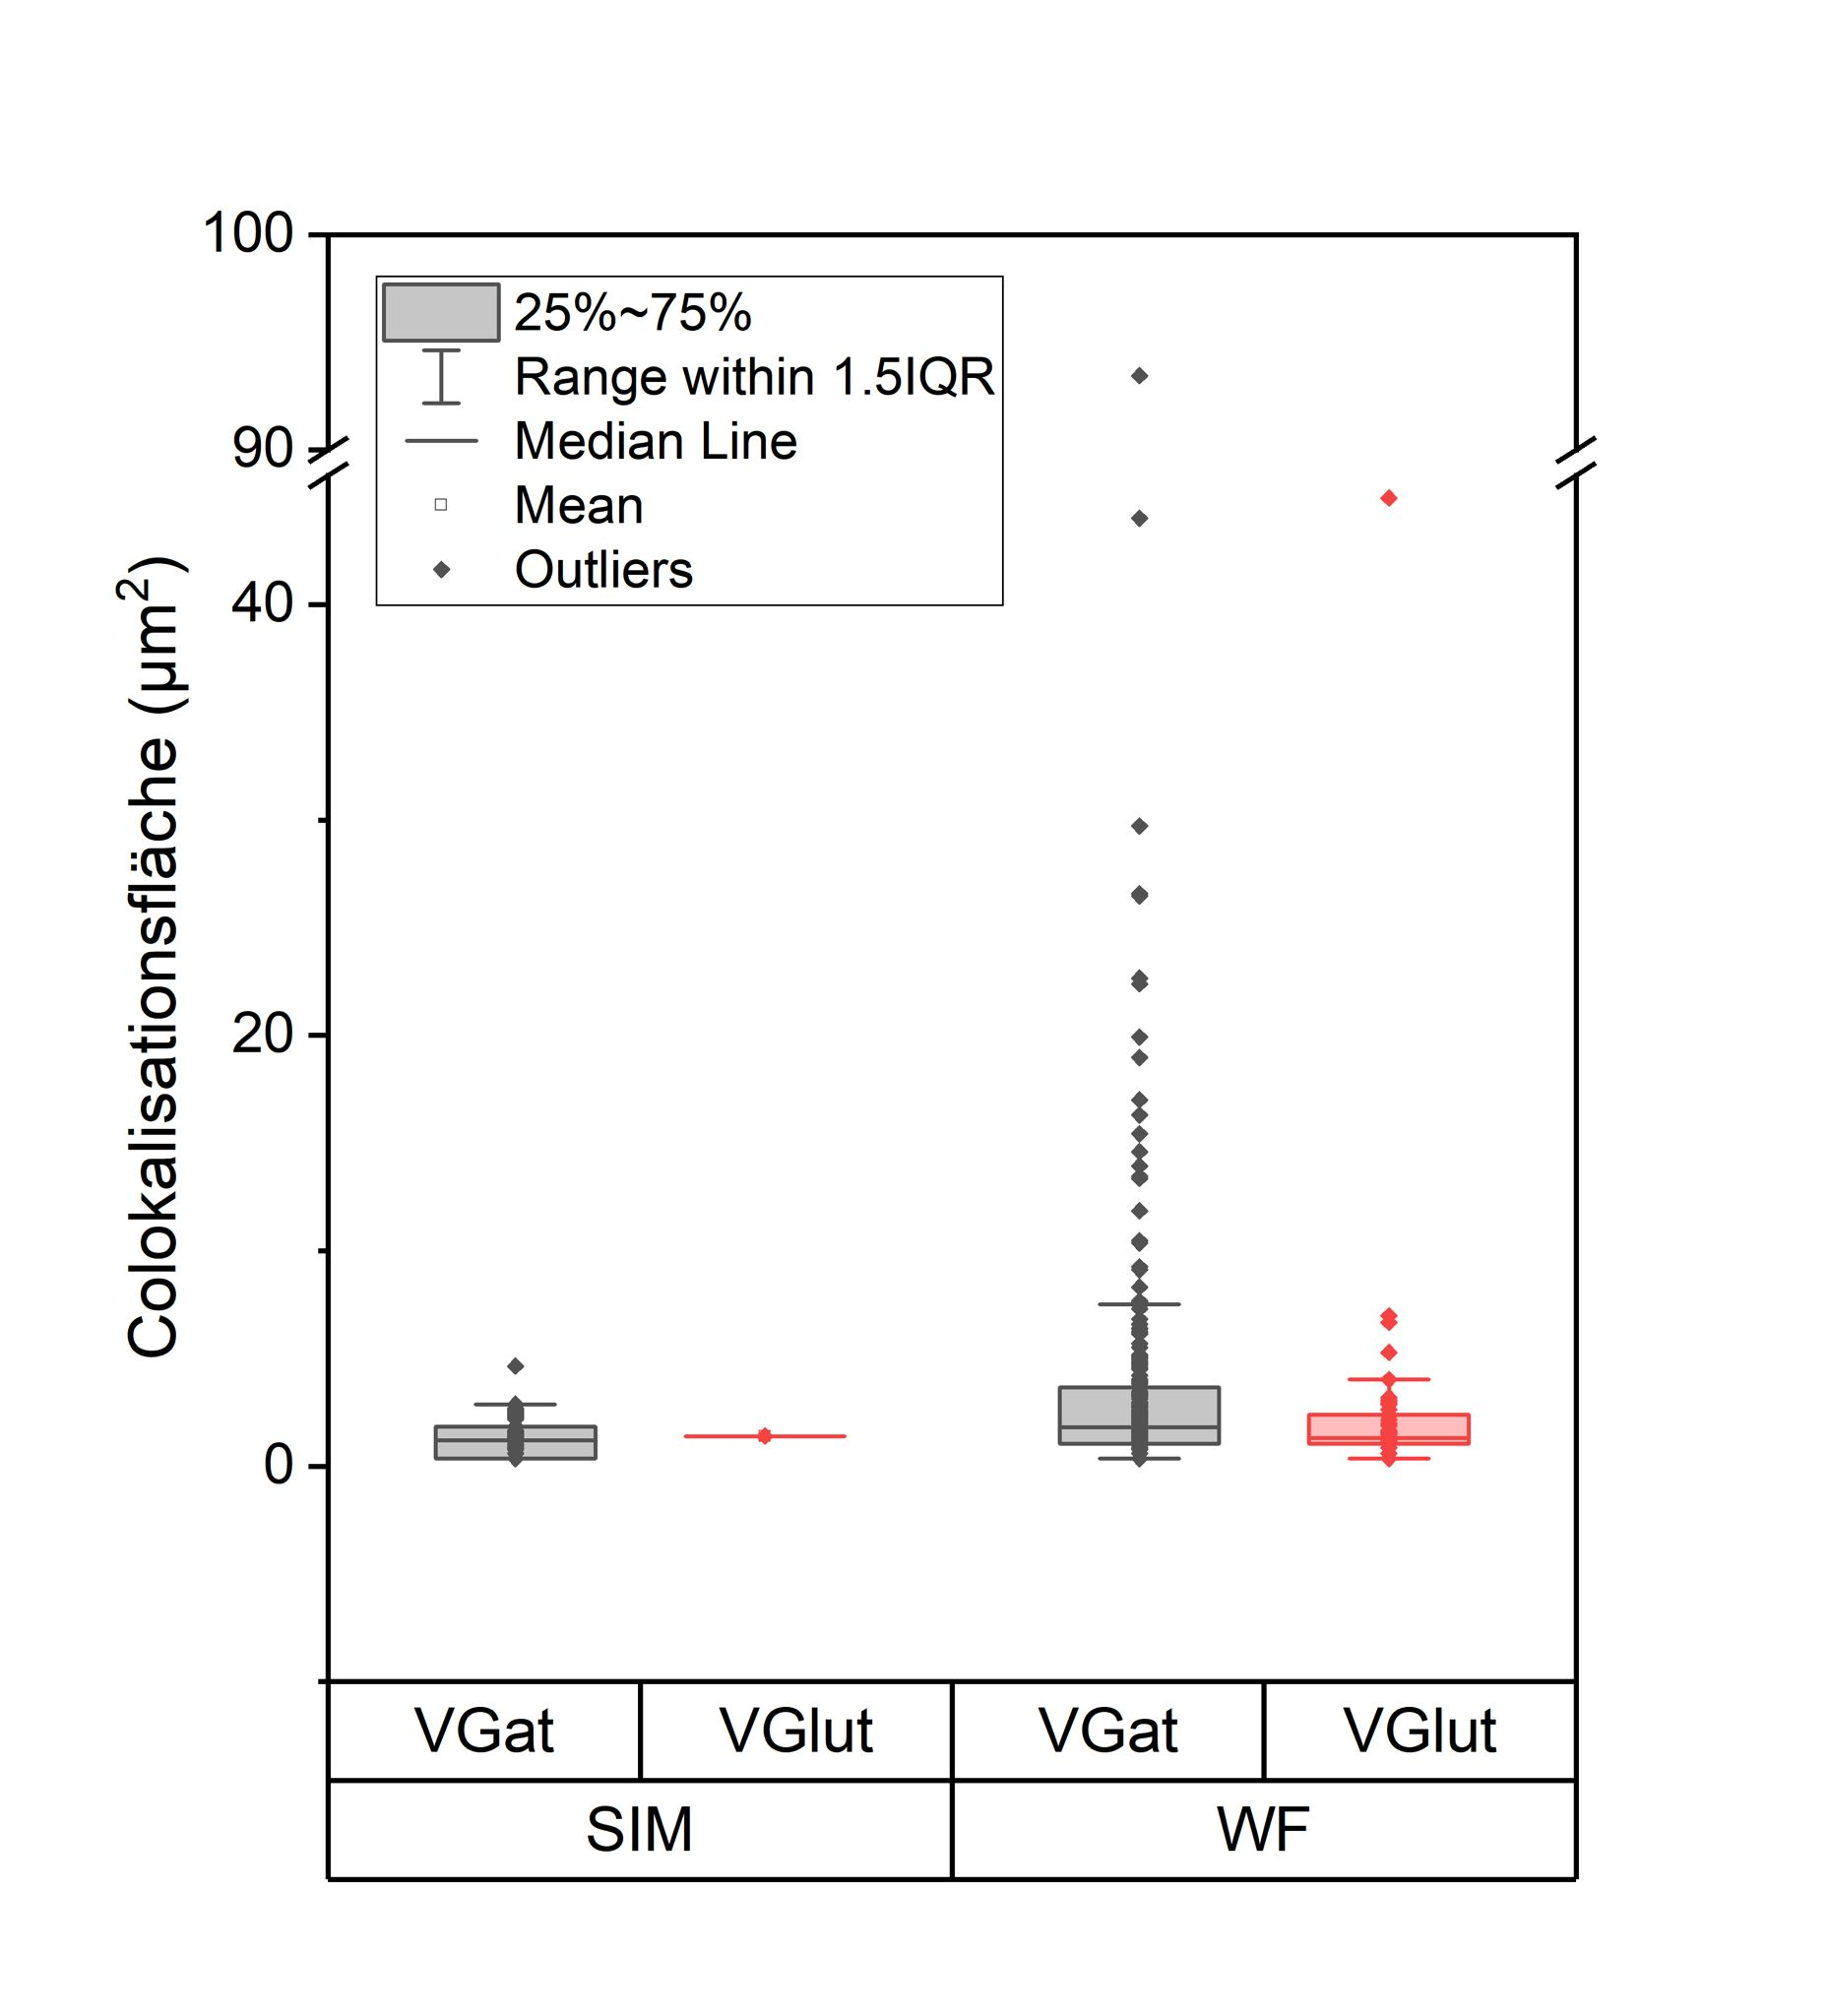
\includegraphics[width=0.8\textwidth]{abbildungen/colokflächemarkerKCVV.jpg} % Lädt das Bild, skaliert es auf 80% der Textbreite
	\caption{Colokalisationsfläche von Caspr2 mit synaptischen
		Markern VGlut und VGat \parencite{eigenAu7.1}} % Die Bildunterschrift
	\label{fig:coflma} % Ein Label für Querverweise (z.B. "siehe Abbildung \ref{fig:beispielbild}")
\end{figure}
\begin{figure}[h] % [h] versucht, das Bild hier zu platzieren (hier), [t] für oben, [b] für unten
	\centering % Zentriert das Bild horizontal
	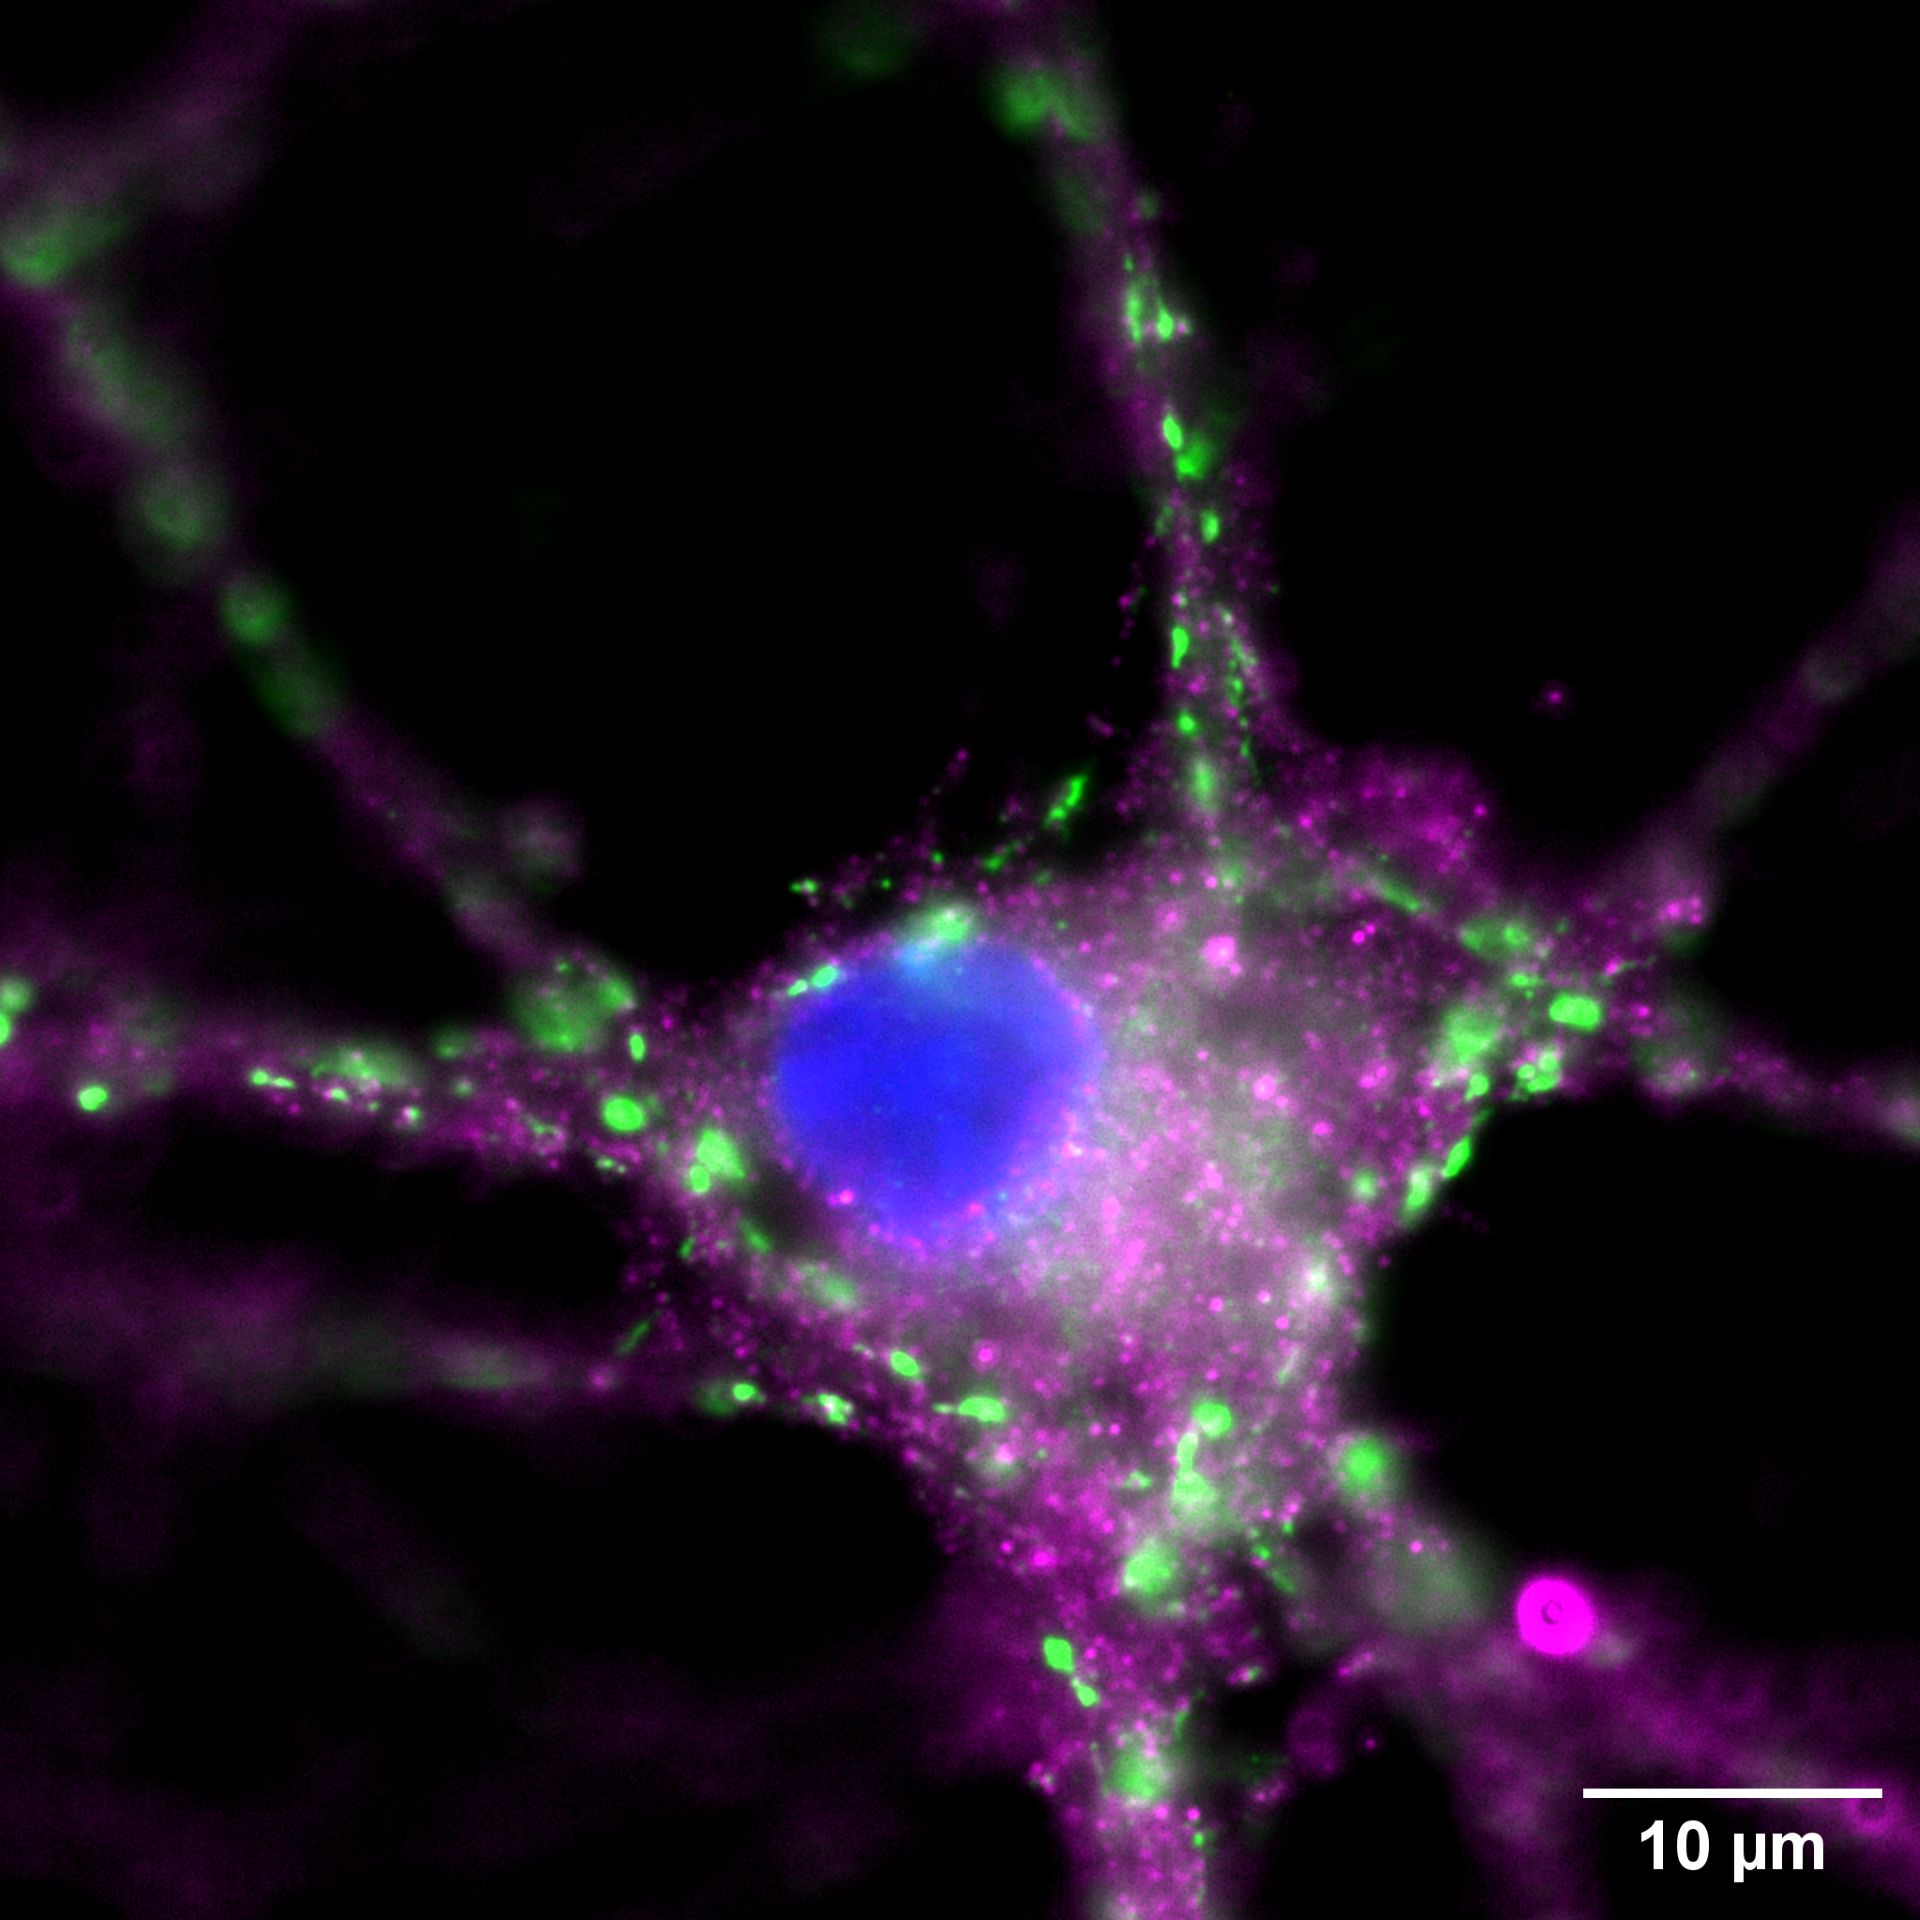
\includegraphics[width=0.8\textwidth]{abbildungen/WFNervEuA.png} % Lädt das Bild, skaliert es auf 80% der Textbreite
	\caption{Wide-Field-(WF)-Aufnahme einer Nervenzelle. Die fluoreszierenden Strukturen zeigen Caspr2 (magenta), VGat (grün) und einen Zellkern (blau) \parencite{eigenAu7.2}} % Die Bildunterschrift
	\label{fig:WFnerv} % Ein Label für Querverweise (z.B. "siehe Abbildung \ref{fig:beispielbild}")
\end{figure}
\begin{figure}[h] % [h] versucht, das Bild hier zu platzieren (hier), [t] für oben, [b] für unten
	\centering % Zentriert das Bild horizontal
	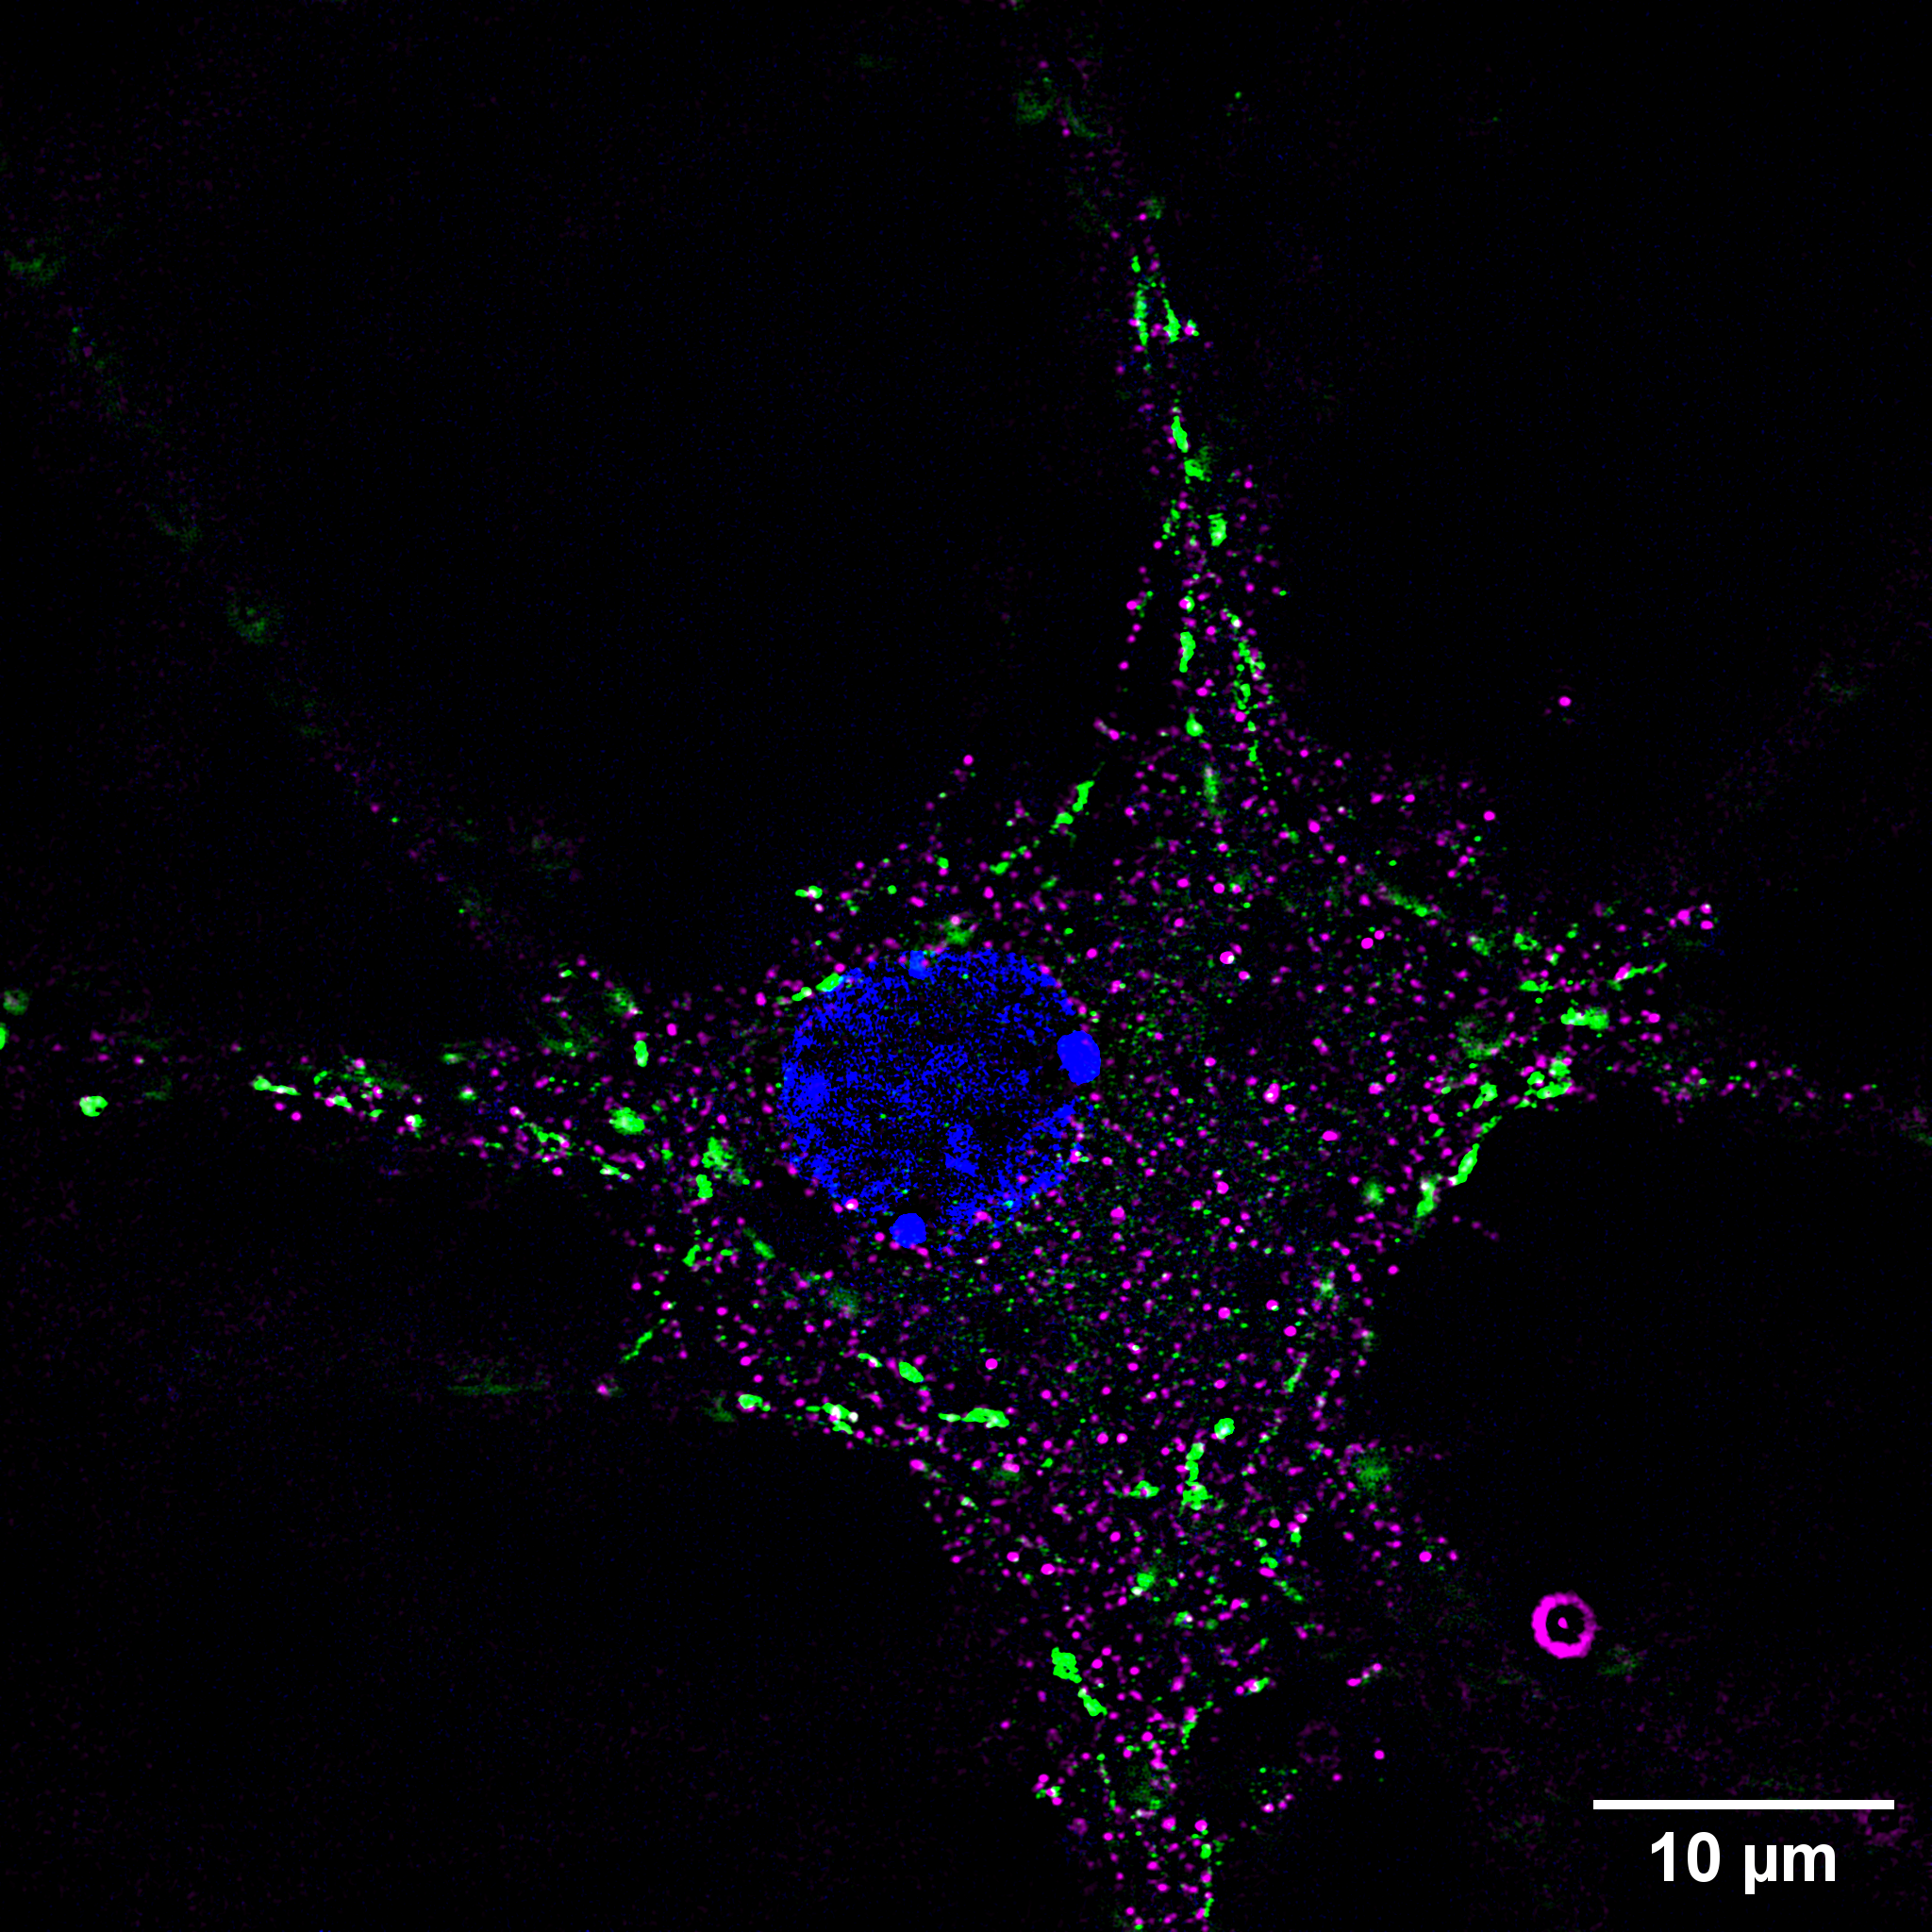
\includegraphics[width=0.8\textwidth]{abbildungen/SIMNervEuA.png} % Lädt das Bild, skaliert es auf 80% der Textbreite
	\caption{Structured-Illumination-Microscopie-(SIM)-Aufnahme einer Nervenzelle. Die fluoreszierenden Strukturen zeigen Caspr2 (magenta), VGat (grün) und einen Zellkern (blau) \parencite{eigenAu7.3}} % Die Bildunterschrift
	\label{fig:SIMnerv} % Ein Label für Querverweise (z.B. "siehe Abbildung \ref{fig:beispielbild}")
\end{figure}
% ── Abbildung 2 (Mann-Whitney U-Test Screenshot) ausgelassen ─
% Abb. 2: Mann-Whitney U-Test von SIM in OriginPro 2019
% 
%%	\centering % Zentriert das Bild horizontal
%	\label{fig:mwutma} % Ein Label für Querverweise (z.B. "siehe Abbildung \ref{fig:beispielbild}")
%\end{figure}
\clearpage
\section{Kolokalisation von Caspr2 und Contactin-2 nach der
	Behandlung mit verschiedenen Antikörpern}

Zur Untersuchung des Effekts der Anti-Caspr2-aAK auf die Interaktion
zwischen Caspr2 und Contactin-2 wurden Neuronenkulturen von Mäusen
entweder mit AK gegen die Discoidin- oder die Laminin-Domäne von Caspr2
behandelt. Mittels SIM wurden hochauflösende Aufnahmen der Synapsen gemacht. Die Kolokalisationsflächen wurden mittels IMARIS analysiert.

Bei der Überprüfung der Werte mittels Shapiro-Wilk-Tests lag keine
Normalverteilung vor, daher erfolgte erneut ein Vergleich zwischen den
Gruppen mittels Mann-Whitney U-Test.

Die Kolokalisationsflächen in Abbildung \ref{fig:aAKstat} weisen in beiden Gruppen ähnliche Wertebereiche auf. Bei den Antikörpern, die an die Discoidin-Domäne
binden, liegt der Median bei ca.\ $1{,}8\,\mu\text{m}^2$, die mittleren
50\,\% der Werte liegen in etwa zwischen
$1{,}4$--$2{,}5\,\mu\text{m}^2$ und es liegt ein Wert außerhalb des
Hauptbereichs bei rund $5\,\mu\text{m}^2$.

Die Laminin-Werte sind zahlreicher und deutlich stärker gestreut. %...............(diskussion dann später)
Der Median der Laminin-Werte liegt bei
$1{,}6\,\mu\text{m}^2$. Die mittleren 50\,\% der Werte liegen im
Vergleich zu den Discoidin-Werten in einem geringeren Bereich. Der
Bereich reicht von etwa $1{,}2$--$2{,}2\,\mu\text{m}^2$.

Der Mann-Whitney U-Test zeigt keinen signifikanten
Unterschied zwischen den Werten von AK, die an die Discoidin- oder
Laminin-Domäne binden ($p = 0{,}386$, n.\,s.).

Der Mann-Whitney U-Test liefert keinen statistischen Nachweis für einen unterschiedlichen Effekt der AK-Gruppen. Eine mögliche Tendenz ist aufgrund vermehrter Einzelwerte und einer größeren Streuung der Werte in den Proben der Laminin-AK zu vermuten. Dennoch lässt sich hier keine eindeutige Aussage treffen.

% ── Abbildung 3 (Boxplot Discoidin/Laminin) ausgelassen ──────
% Abb. 3: Einfluss von Anti-Caspr2-aAK gegen die Discoidin-
%         bzw. Laminin-Domäne von Caspr2 auf die Kolokalisation
%         mit Contactin-2
% ─────────────────────────────────────────────────────────────
\begin{figure}[h] % [h] versucht, das Bild hier zu platzieren (hier), [t] für oben, [b] für unten
	\centering % Zentriert das Bild horizontal
	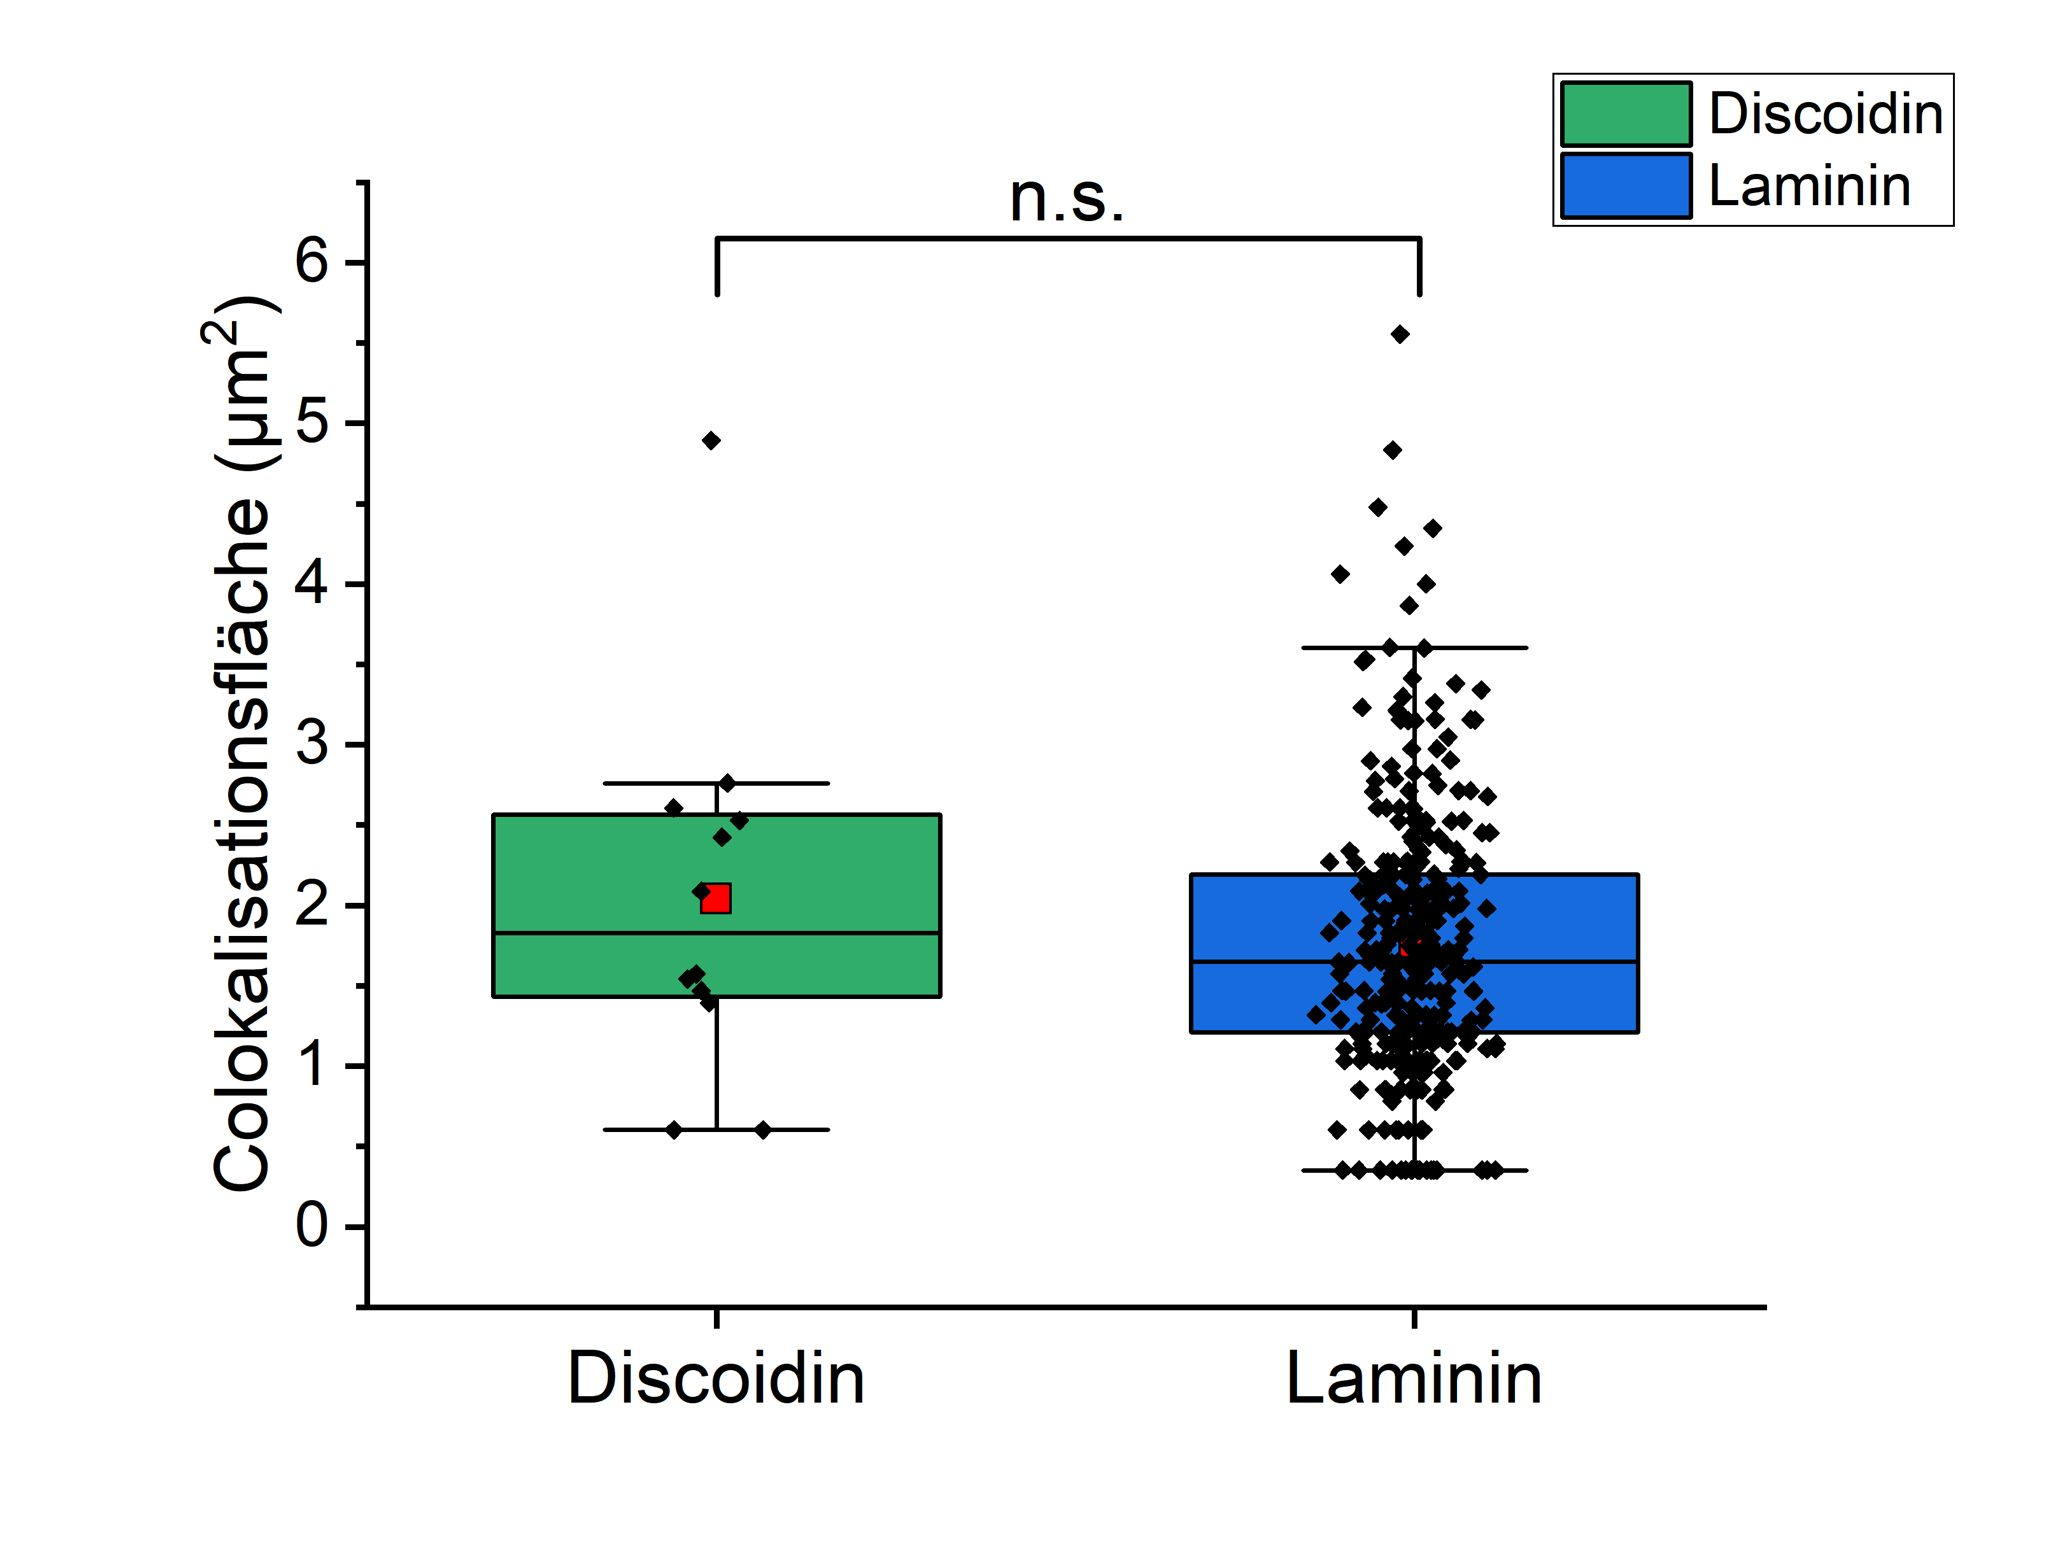
\includegraphics[width=0.91\textwidth]{abbildungen/aAKstatKCVV.jpg} % Lädt das Bild, skaliert es auf 80% der Textbreite
	\caption{Einfluss von Anti-Caspr2-aAK gegen die Discoidin- bzw. Laminin-Domäne
		von Caspr2 auf die Kolokalisation mit Contactin-2 \parencite{eigenAu7.4}} % Die Bildunterschrift
	\label{fig:aAKstat} % Ein Label für Querverweise (z.B. "siehe Abbildung \ref{fig:beispielbild}")
\end{figure}

% ── Abbildung 4 (Mann-Whitney U-Test Screenshot) ausgelassen ─
% Abb. 4: Mann-Whitney U-Test in OriginPro 2019
% ─────────────────────────────────────────────────────────────
%\begin{figure}[h] % [h] versucht, das Bild hier zu platzieren (hier), [t] für oben, [b] für unten
%	\centering % Zentriert das Bild horizontal
%	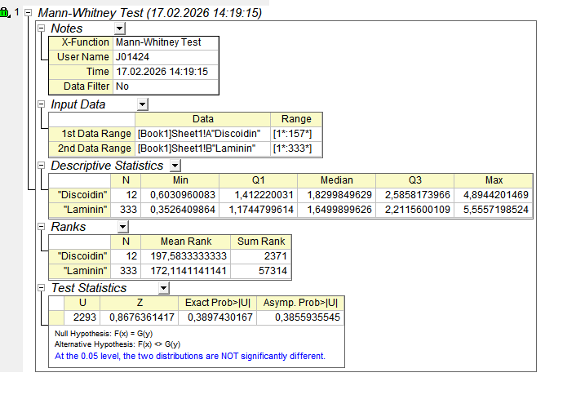
\includegraphics[width=0.91\textwidth]{abbildungen/mwutestaAK.png} % Lädt das Bild, skaliert es auf 80% der Textbreite
%	\caption{Mann-Whitney U-Test von SIM in OriginPro 2019 auf der Einfluss von Anti-Caspr2-aAK \parencite{eigenAu7.4}} % Die Bildunterschrift
%	\label{fig:mwutaAK} % Ein Label für Querverweise (z.B. "siehe Abbildung \ref{fig:beispielbild}")
%\end{figure}
 
\clearpage
%Um die Lokalisation zu bestimmen, wurde jeweils Caspr2 und vesikuläre
%GABA-Transporter (VGat) oder vesikuläre Glutamattransporter (VGlut)
%angefärbt. VGat dient dabei als Marker für inhibitorische Synapsen und
%VGlut als Marker für exzitatorische Synapsen. Mittels Bestimmung der
%Kolokalisationsfläche der fluoreszierenden Farbstoffe lässt sich
%ermitteln, an welcher Synapsenart Caspr2 vorwiegend vorliegt.
%
%In Abb.~1 ist jeweils die Größe einzelner sowie die Anzahl an
%Kolokalisationsflächen ($\mu\text{m}^2$) von Caspr2 mit den
%Synapsenmarkern VGat (schwarz) und VGlut (rot) bei den
%Mikroskopieverfahren Structured Illumination Microscopy (SIM) und Wide
%Field (WF) dargestellt.
%
%Die durchschnittliche Kolokalisationsfläche von VGat ist bei der
%SIM-Mikroskopie ähnlich groß wie die VGlut-Kolokalisationsfläche und
%liegt bei ca.\ $1\,\mu\text{m}^2$. Die Kolokalisationsflächen von Caspr2
%und VGat sind teils größer und es wurden deutlich mehr
%Kolokalisationsflächen gefunden. Bei der VGlut-Analyse findet sich
%lediglich ein Wert.
%% Anmerkung: Färbung hat nicht sonderlich gut funktioniert – 
%%            Fehlerbetrachtung einfügen.
%
%Bei der WF-Mikroskopie lässt sich eine starke Streuung der Größe der
%Kolokalisationsflächen von VGat und Caspr2 finden. Des Weiteren liegen
%teilweise sehr große Kolokalisationsflächen vor. Der Median der
%VGat-Kolokalisation ist minimal höher als der der VGlut-Kolokalisation,
%beide liegen im Bereich von ca.\
%$1{,}5$--$2\,\mu\text{m}^2$. Die Größen der
%VGlut-Kolokalisationsflächen liegen im moderaten Bereich und weisen eine
%geringere Streuung als bei VGat auf. Sowohl bei der WF- als auch bei der
%SIM-Mikroskopie ist die Anzahl an Kolokalisationsflächen bei VGat
%erkennbar höher.
%
%Die erhöhte Anzahl an VGat-Kolokalisation ist im Kontext zu sehen. Die
%Synapsendichte an inhibitorischen Synapsen könnte in den Aufnahmen größer
%gewesen sein als die der exzitatorischen Synapsen. Die Mediane der
%Flächengrößen sind annähernd gleich.